\documentclass[12pt]{article}
\usepackage[utf8]{inputenc}
\usepackage{hyperref}
\usepackage{graphicx}

\title{Weather Report for Freiburg}
\date{}

\begin{document}
\maketitle
\section*{Weather at a Glance }
At a cool 11.0°C, the air whispers of change, brisk and refreshing. It hints at the need for a warm layer, inviting a sense of calm and a breath of fresh air. This gentle reminder of the season's shift encourages one to savor the crispness that envelops the surroundings. Above, the skies of Freiburg don a cloak of partly cloudy, setting the stage for the day's mood. A wind, carrying whispers at 20.2 kph from the SSW, shapes the air's embrace. The atmosphere, pressing down with a pressure of 996.0 mb, remains unseen but deeply felt, a silent guardian of the day. Humidity at 66% weaves a tale of invisible waters binding earth and sky, while clouds, those fleeting masterpieces, adorn 75% of the heavens. This dance of light and shadow plays over the landscape, with the mercury hinting at 11.0°C yet the sensation on the skin echoes 8.9°C. Visibility stretches to 10.0 km, promising clear views that invite the soul to wander. Together, these elements weave a tapestry of weather in Freiburg, not merely a story of data but an experience woven from the sun's warmth, the wind's caress, and the clouds' silent passage. Here, in the heart of Freiburg, the day unfolds with a promise of moments lived under an ever-changing sky, a narrative rich with the essence of life itself.
\paragraph{}This graph provides a clear idea about the temperature and precipitation in Freiburg.
\begin{figure}[h]
\centering
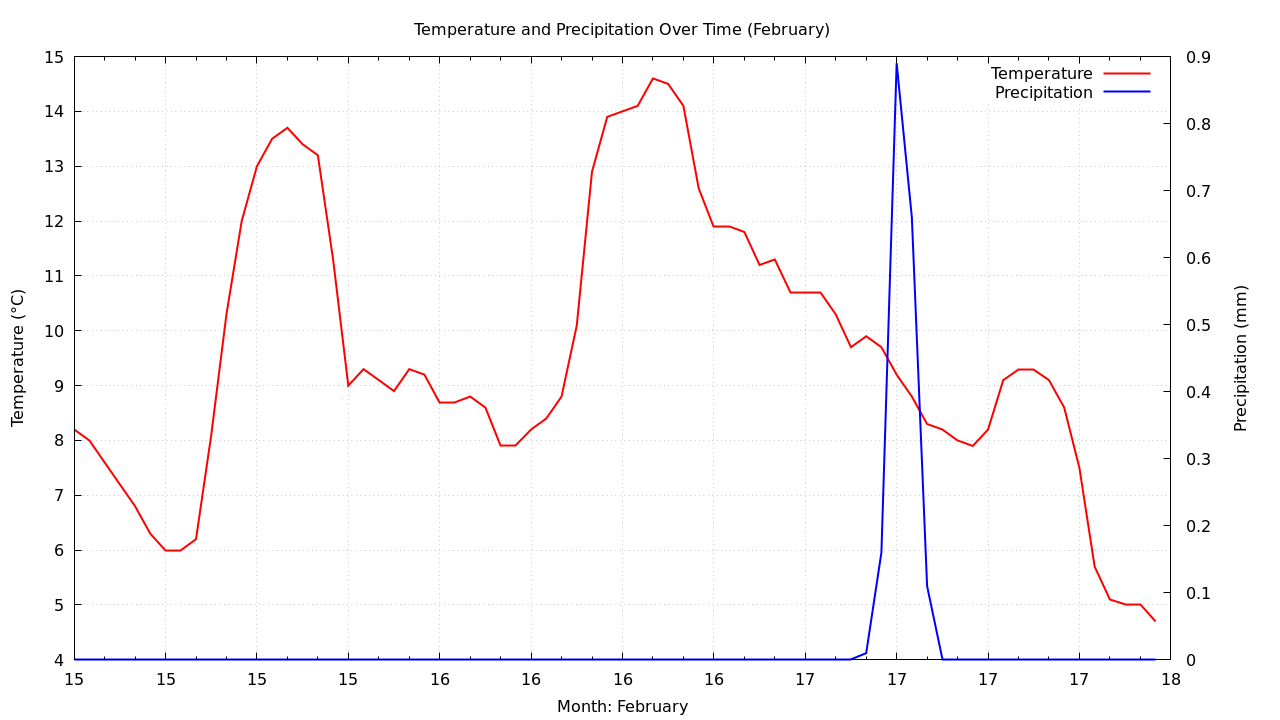
\includegraphics[width=0.8\textwidth]{data/graph/temperature_precipitation_graph.png}
\caption{Temperature and Precipitation Overview in Freiburg}
\end{figure}

\end{document}